\documentclass{article}
\usepackage{iclr2027_conference,times}

\input{math_commands.tex}

\usepackage{graphicx}
\usepackage{caption}
\usepackage{subcaption}
\usepackage{booktabs}
\usepackage{multirow}
\usepackage{array}
\usepackage{makecell}
\usepackage{siunitx}
\sisetup{
  group-separator={,},
  group-minimum-digits=4,
  table-number-alignment=center,
  detect-weight=true,
  detect-inline-weight=math,
}
\usepackage{microtype}
\usepackage{hyperref}
\usepackage{url}
\usepackage{etoolbox}
\usepackage{wrapfig}
\usepackage{placeins}

% Float/caption spacing; Fig.~3--4 use \pairedfigrow and \pairedfigcaption.
\setlength{\textfloatsep}{8pt plus 2pt minus 2pt}
\setlength{\floatsep}{8pt plus 2pt minus 2pt}
\setlength{\intextsep}{8pt plus 2pt minus 2pt}
\setlength{\abovecaptionskip}{0pt}
\setlength{\belowcaptionskip}{2pt}
\captionsetup{skip=1pt}
\captionsetup[subfigure]{skip=1pt}
\captionsetup[subtable]{skip=1pt}
\newcommand{\floatbodycaptionskip}{\vspace{-5pt}}
\newcommand{\floattablecaptionskip}{\vspace{-5pt}}
\pretocmd{\caption}{\floatbodycaptionskip}{}{}
\newcommand{\floatstacksep}{\vspace{6pt}}
\newcommand{\benchmarkstacksep}{\vspace{5pt}}

% Floats may share pages with body text above and below (table + figure in §2.2).
% Allow the compact ablation tables and paired analysis figures to share page 8.
\setcounter{topnumber}{2}
\setcounter{bottomnumber}{2}
\setcounter{totalnumber}{4}
\renewcommand{\bottomfraction}{0.65}
\renewcommand{\floatpagefraction}{0.85}

\title{Charts as Epistemic Actions: Experience-Driven Chart Use in Agentic Data Analysis}

% Keep the submission anonymous. Do not uncomment \iclrfinalcopy.
\author{Anonymous Authors}

\newcommand{\method}{\textsc{Ours}}
\newcommand{\probe}{\textsc{ProbeTask}}
\newcommand{\na}{\textemdash}
\newcommand{\headpct}{(\%)}
\newcommand{\tabmethodreported}[1]{\makecell[l]{#1\\(reported)}}
\newcommand{\tabmethodbaseline}{\makecell[l]{Baseline\\(ReAct,\\Reproduced)}}
\newcommand{\placeholderfigure}[2]{%
  \fbox{\begin{minipage}[c][#1][c]{0.94\linewidth}
    \centering\small\textbf{#2}\\[0.5em]
    Final source figure not yet available.
  \end{minipage}}}
% Side-by-side figures (Fig.~3--4): two equal-height panels in one shared float.
\newlength{\pairedfigpanelheight}
\newlength{\pairedfigplaceholderheight}
\setlength{\pairedfigpanelheight}{4.5cm}
\setlength{\pairedfigplaceholderheight}{\dimexpr\pairedfigpanelheight-2\fboxsep-2\fboxrule\relax}
\newcommand{\pairedfiggraphicarea}[1]{%
  \parbox[c][\pairedfigpanelheight][c]{\linewidth}{\centering #1\par}%
}
\newcommand{\pairedfigplaceholder}[1]{%
  \pairedfiggraphicarea{%
    \fbox{\begin{minipage}[c][\pairedfigplaceholderheight][c]{\dimexpr0.82\linewidth-2\fboxsep-2\fboxrule\relax}
      \centering\small\textbf{#1}\\[0.4em]
      Final source figure not yet available.
    \end{minipage}}%
  }%
}
\newcommand{\pairedfiginclude}[1]{%
  \pairedfiggraphicarea{%
    \includegraphics[width=0.82\linewidth,height=\pairedfigpanelheight,keepaspectratio]{#1}%
  }%
}
% Optional arg: \pairedfigcaption[label]{caption text}
\newcommand{\pairedfigcaption}[2][]{%
  \par\vspace{5pt}%
  \begingroup
  \captionsetup{skip=2pt,width=\linewidth,justification=centering,singlelinecheck=false}%
  \caption{#2}%
  \ifx\relax#1\relax\else\label{#1}\fi
  \endgroup
}
\newcommand{\pairedfigrow}[2]{%
  \WFclear
  \begin{figure}[!t]
    \centering
    \begin{minipage}[t]{0.48\textwidth}
      \vspace{0pt}\centering
      #1
    \end{minipage}\hfill
    \begin{minipage}[t]{0.48\textwidth}
      \vspace{0pt}\centering
      #2
    \end{minipage}
  \end{figure}%
}

\begin{document}

\maketitle

\begin{abstract}

  % 图表是人类分析师识别趋势、模式和异常的重要认知工具。尽管数据智能体能够生成和解读图表，但图表对于智能体数据分析的实际效用仍缺乏深入研究。在本文中，我们首先基于标注问题设计了一项探究实验，考察智能体解读图表证据的能力及其在开放式自主分析中的图表使用行为。我们发现，受评测智能体能有效地从图和表中提取分析证据，但在自主分析中是否主动使用图表方面存在显著差异。此外，图表与文本呈现出任务依赖的能力互补性。上述结果表明，图表不应仅被视为事后呈现工具，而应成为数据智能体推理过程的内在组成部分。基于这一认识，我们进一步提出一种经验驱动方法，通过对条件化分析轨迹进行评分与归因，提炼分析经验与表征经验，帮助智能体学习如何构建、选择和使用图表证据，并缓解其表征使用偏置。在三个基准上的实验表明，该方法能够促进智能体主动利用图表开展分析，并显著优于基线方法。
  
  Charts are important cognitive tools that help human analysts identify trends, patterns, and anomalies. Although data agents can generate and interpret charts, the analytical utility of charts in agentic data analysis remains underexplored. In this work, we first conduct a probe study based on annotated questions to examine agents' ability to interpret chart evidence and their chart-use behavior in open-ended analysis. We find that the evaluated agents effectively extract useful evidence from charts and tables, but differ substantially in whether they actively use charts during analysis. Moreover, charts and text exhibit task-dependent complementarity. These findings suggest that charts should not serve merely as post-hoc presentation tools, but should form an intrinsic part of data agents' reasoning. Building on this insight, we propose an experience-driven method for chart use in agentic data analysis. The method distills analysis and representation experiences from conditioned trajectory rollouts using outcome scores and step-level attributions. The validated experience package helps agents learn how to construct, select, and use chart evidence while mitigating representation-use biases. Experiments on three held-out benchmarks show that our method encourages agents to actively use charts for analysis and significantly outperforms baseline methods.
\end{abstract}

\section{Introduction}
\label{sec:introduction}

Data agents transform analytical goals into sequences of data-grounded actions and insights.
Advances in ReAct-style reasoning--acting loops and tool use~\citep{yao2023react} enable these agents to plan, execute, inspect, and revise increasingly complex analytical workflows.

Despite this progress, most ReAct-style data agents remain text-centric.
SQL queries and Python programs specify analytical operations, but their results are typically converted into textual observations before being returned to the agent.
Human analysts work differently, moving repeatedly between numerical summaries, tables, and charts to expose different evidence and guide subsequent operations.
This contrast creates a fundamental gap between current data agents and human analysis.
It raises a central question for agentic data analysis, whether an agent should rely on text, use charts as human analysts do, or choose between them as the analysis unfolds.

Existing methods address only parts of this decision.
Most data agents reason over textualized execution results and use charts primarily as final report artifacts.
Chart-generation methods optimize visualizations requested by a user or an agent~\citep{dibia2023lida,yang2024matplotagent,yang2025chartmimic,namgoong2025amace,lu2026multivisagent,wang2025chartoptimiser}, whereas chart-understanding methods assume that a chart is already available and focus on extracting information from it~\citep{masry2023unichart,han2023chartllama,xu2023chartbench,liu2023deplot,liu2023matcha,zhang2024tinychart}.
Recent studies introduce visual representations into reasoning or select among predefined formats~\citep{kaur2026chartagent,das2025chartsofthought,zhou2025fres,ho2026formatmatters,xing2026tabledart,lin2026evidfuse}, but chart use remains prescribed, dependent on agent-specific preferences, or disconnected from the current analysis state.
Consequently, existing methods do not provide a reliable mechanism for choosing between text and chart evidence during open-ended analysis.

An effective data agent should select both the analytical operation and the evidence representation that best fit the question and current analysis state.
Before designing such an agent, we must establish whether charts provide genuine analytical value, how their utility differs from text, and whether current agents exhibit a gap between understanding charts and using them effectively.
We therefore construct \probe{} to evaluate agents under controlled text and chart interfaces across analytical tasks and cognitive demands.
Two main findings emerge.
First, agents can extract sufficient evidence from charts, yet access to plotting tools does not produce reliable chart use, revealing a pronounced \emph{capability--utility} gap.
Second, charts and text serve as complementary evidence representations, with charts supporting trends, patterns, and anomalies, and text supporting precise reading, conditional verification, and evidence integration.

Motivated by these findings, we propose an experience-driven method for chart use in agentic data analysis.
For each \probe{}, the method generates conditioned trajectory rollouts and uses outcome scores and step-level attributions to distill an experience package.
The package contains analysis experience for selecting and verifying analytical operations, and representation experience for deciding when and how intermediate evidence should use text, charts, or both.
Candidate packages are retained only when they improve validation performance.
During downstream analysis, the frozen experience package guides the agent in selecting analytical operations and evidence representations without fixed representation-selection rules.

In summary, our main contributions are as follows:
\begin{itemize}
  \item We systematically probe the analytical utility of charts for data agents on synthetic trajectories (\probe{}), revealing a gap between chart understanding and productive use of open plotting, and summarizing task-dependent complementarity between charts and text as evidence representations.
  \item We propose an experience-driven method that distills analysis and representation experiences from conditioned trajectory rollouts with outcome scores and step-level attributions, enabling agents to learn both what evidence to construct and how to represent and use it without fixed representation-selection rules.
  \item Experiments on three external data-analysis benchmarks (DAComp-DA, DDR-Bench, and DSBench) with six LLM backbones demonstrate that our method consistently outperforms matched baseline agents; ablations on single experience types, chart disabling, and a fixed experience package quantify the contribution of experience distillation and visual representation.
\end{itemize}



\section{Charts in the Analytical Loop}
\label{sec:probe}

We use \probe{} to determine whether charts provide genuine analytical value to data agents and how their utility differs from text.
We first describe the probe design and evaluation protocol, then examine chart-based analysis, open-ended representation choice, and the complementary strengths of text and charts.

\subsection{Probe Design}
\label{sec:probe-setup}

\noindent\textbf{Task construction.}
To isolate how intermediate representations affect agent reasoning, we synthesize \probe{} from InsightBench~\citep{sahu2025insightbench}, which provides enterprise tables, open-ended questions, executable reference analyses, and target insights.
From the first 50 source-data flags of InsightBench, we synthesize 200 \probe{} tasks by treating each valid insight as an independent task.
Each task contains a raw CSV table, dataset description, analytical question, reference analysis, and target insight.
The agent receives the table, question, description, schema, and first three rows, while the target insight remains hidden for evaluation; it must select and execute the required operations and return a direct natural-language answer.

\noindent\textbf{Annotations and evaluation.}
We annotate each task along two complementary dimensions for post-hoc analysis.
\emph{Question type} describes the requested answer, including numeric lookup, composition, rank or extreme, group comparison, temporal change, relationship, anomaly or risk, diagnosis, and prediction; \emph{cognitive load} describes the primary operation, including locate, scan and select, compare, recognize a pattern, interpret a relation, integrate dimensions, and conditional reasoning.
An LLM assigns the initial labels and a human annotator reviews them; these labels support slice analysis only and never define representation-selection rules.
A common GPT-5.6 Sol judge scores each answer against the question and target insight on a 0--4 scale, and we report the mean normalized score on $[0,100]$.
Slice analyses use task-paired differences with flag-clustered bootstrap intervals~\citep{efron1993bootstrap} and randomization tests.

\noindent\textbf{Agent interfaces.}
All settings share the same vanilla ReAct agent with one general-purpose Bash tool.
Each call starts a fresh process, while files persist in a shared working directory and the CSV is exposed read-only.
We hold the task, model, initial context, interaction limit, and tool budget fixed across groups; only the analytical interface differs.
\textbf{No-tool} removes execution tools, \textbf{Text-only} exposes stdout and stderr but prohibits plotting, \textbf{Chart-only} exposes generated images and stderr while hiding stdout, and \textbf{Free-style} returns stdout, stderr, and images and permits both text and charts.

On the full suite ($n{=}200$), we run an interface ablation with GPT-5.6 Sol across all four settings and compare six model backbones under Free-style; Tables~\ref{tab:four-condition} and~\ref{tab:model-bias} report the corresponding results.
The same GPT-5.6 Sol judge scores all runs.


\begin{table}[t]
	\centering
	\vspace{-4pt}
	\hfill
	\begin{minipage}[t]{0.33\textwidth}
		\centering
		\scriptsize
		\captionsetup{width=\linewidth,justification=centering,singlelinecheck=false}%
		\captionof{table}{Interface ablation on \probe{} with\\GPT-5.6 Sol.}
		\label{tab:four-condition}
		\begin{tabular}{@{}lr@{}}
			\toprule
			Interface & Score \\
			\midrule
			No-tool & 29.4 \\
			Text-only & 77.2 \\
			Chart-only & 78.4 \\
			Free-style & 77.6 \\
			\bottomrule
		\end{tabular}
	\end{minipage}\hfill
	\begin{minipage}[t]{0.53\textwidth}
		\centering
		\captionsetup{width=\linewidth,justification=centering,singlelinecheck=false}%
		\captionof{table}{Free-style results across six LLM backbones.}
		\label{tab:model-bias}
		{\setlength{\tabcolsep}{2.6pt}%
			\renewcommand{\arraystretch}{1.12}%
			\scriptsize
			\begin{tabular}{@{}lcccccc@{}}
				\toprule
				\multirow{2}{*}[-0.15em]{LLM backbone} &
				\multirow{2}{*}[-0.15em]{Score} &
				\multicolumn{3}{c}{Representation use (\# tasks)} &
				\multicolumn{2}{c}{ReAct cost} \\
				\cmidrule(lr){3-5}%
				\cmidrule(lr){6-7}
				& & Text & Chart & Both & Rounds & Tokens \\
				\midrule
				Claude Opus 5 & 83.1 & 43 & 0 & 157 & 3.9 & 17{,}401 \\
				Claude Sonnet 5 & 79.2 & 102 & 0 & 98 & 4.0 & 18{,}724 \\
				GPT-5.6 Luna & 76.2 & 198 & 0 & 2 & 3.1 & 6{,}835 \\
				GPT-5.6 Sol & 77.6 & 198 & 0 & 2 & 2.9 & 6{,}392 \\
				DeepSeek V4.1 Flash & 80.2 & 143 & 0 & 57 & 6.2 & 30{,}051 \\
				HY3 & 73.1 & 198 & 0 & 2 & 3.8 & 7{,}725 \\
				\bottomrule
		\end{tabular}}
	\end{minipage}\hfill
	\vspace{-10pt}
\end{table}
\vspace{-8pt}

\subsection{Empirical Findings}
\label{sec:probe-findings}

\paragraph{Agents can conduct analysis through charts.}
Table~\ref{tab:four-condition} reports mean scores for the four agent settings.
GPT-5.6 Sol scores 29.4 without tools, 77.2 with text, and 78.4 with charts.
The chart condition performs comparably to text and improves over no-tool by 49.0 points, showing that agents can extract sufficient evidence from charts to answer analytical questions.

\paragraph{Open-ended representation choice exhibits strong model-specific bias.}
Table~\ref{tab:model-bias} compares representation use and interaction cost under the Free-style interface.
Claude Opus 5 combines text and charts on 157 tasks, Claude Sonnet 5 on 98, and DeepSeek V4.1 Flash on 57, whereas GPT-5.6 Luna, GPT-5.6 Sol, and HY3 do so on only 2 tasks each.
Chart-use frequency also has no monotonic relationship with performance, as models with similar use frequencies attain different scores.
Thus, the same text-and-chart interface does not induce a common representation-selection strategy.


\begin{figure}[!tbp]
  \centering
  \begin{subfigure}[t]{\linewidth}
    \centering
    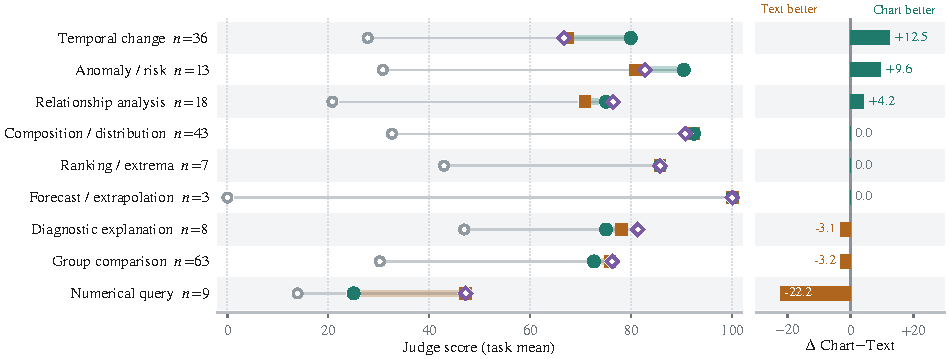
\includegraphics[width=0.82\linewidth]{figures/probe_slices_dotplot_v3_a.pdf}
    \caption{Judge scores by question type.}
    \label{fig:probe-slices-a}
  \end{subfigure}
  \vspace{2pt}
  \begin{subfigure}[t]{\linewidth}
    \centering
    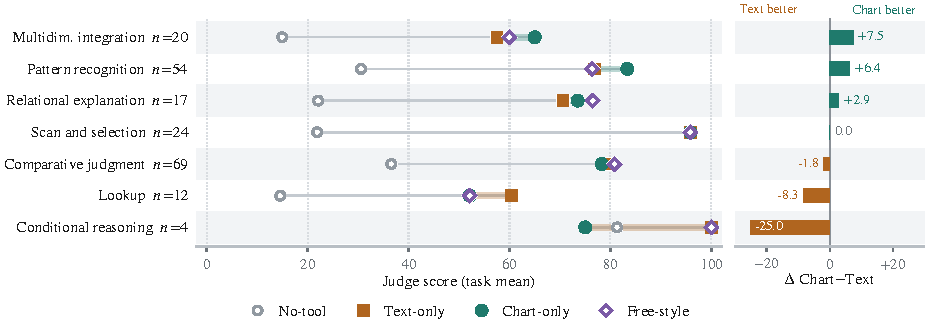
\includegraphics[width=0.82\linewidth]{figures/probe_slices_dotplot_v3_b.pdf}
    \caption{Judge scores by primary cognitive load.}
    \label{fig:probe-slices-b}
  \end{subfigure}
  \caption{Slice analysis of the four agent settings on \probe{} ($n{=}200$).
    Markers show slice means; the right column gives Chart$-$Text $\Delta$ (faded when $n<10$).
    The bottom row of~\subref{fig:probe-slices-a} aggregates all tasks.}
  \label{fig:probe-slices}
\end{figure}

\paragraph{Charts and text exhibit task-dependent complementarity.}
Figure~\ref{fig:probe-slices} breaks down the four settings by question type and cognitive load.
Charts score 0.799 on temporal-change questions, exceeding text by 0.125, and lead by 0.096 on anomaly or risk and by 0.042 on relationship analysis.
They also lead by 0.064 on pattern recognition, by 0.029 on relational explanation, and by 0.075 on multidimensional integration.
The two representations perform similarly on composition or distribution, ranking or extrema, and scan and selection.
Free-style performs below the chart condition on temporal change and pattern recognition, showing that access to both representations does not automatically preserve the benefit of chart evidence.

Text scores 0.472 on numerical queries compared with 0.250 for charts, and 0.604 on lookup tasks compared with 0.521 for charts.
It also leads by 0.032 on group comparison and by 0.018 on comparative judgment.
On conditional reasoning, text scores 1.000 while charts score 0.750, although this slice contains only four tasks.
Text therefore has a relative advantage in exact reading, information location, and conditional verification.

Together, these results reveal a gap between chart-understanding capability and effective chart use.
Agents can extract evidence from self-generated charts, but plotting access alone does not ensure reliable use or coordination with text.
The appropriate representation depends on the task and current analysis state, motivating the experience-driven method developed next.

\FloatBarrier
\section{Learning to Use Charts in Agentic Data Analysis}
\label{sec:method}

We present an experience-driven method that teaches data agents to use charts within the process of agentic data analysis.
The method distills analysis experience and representation experience from trajectories generated under different representation conditions.
The validated experiences then guide the agent in selecting analytical operations and evidence representations, allowing charts to support intermediate reasoning rather than serve only as final outputs.

We first describe the structure and contents of the experience package.
We then present conditioned trajectory rollouts, trajectory scoring and attribution, and the iterative procedure for experience distillation and validation.
Finally, we explain how the resulting experience package guides downstream analysis.

\begin{figure}[!t]
  \centering
  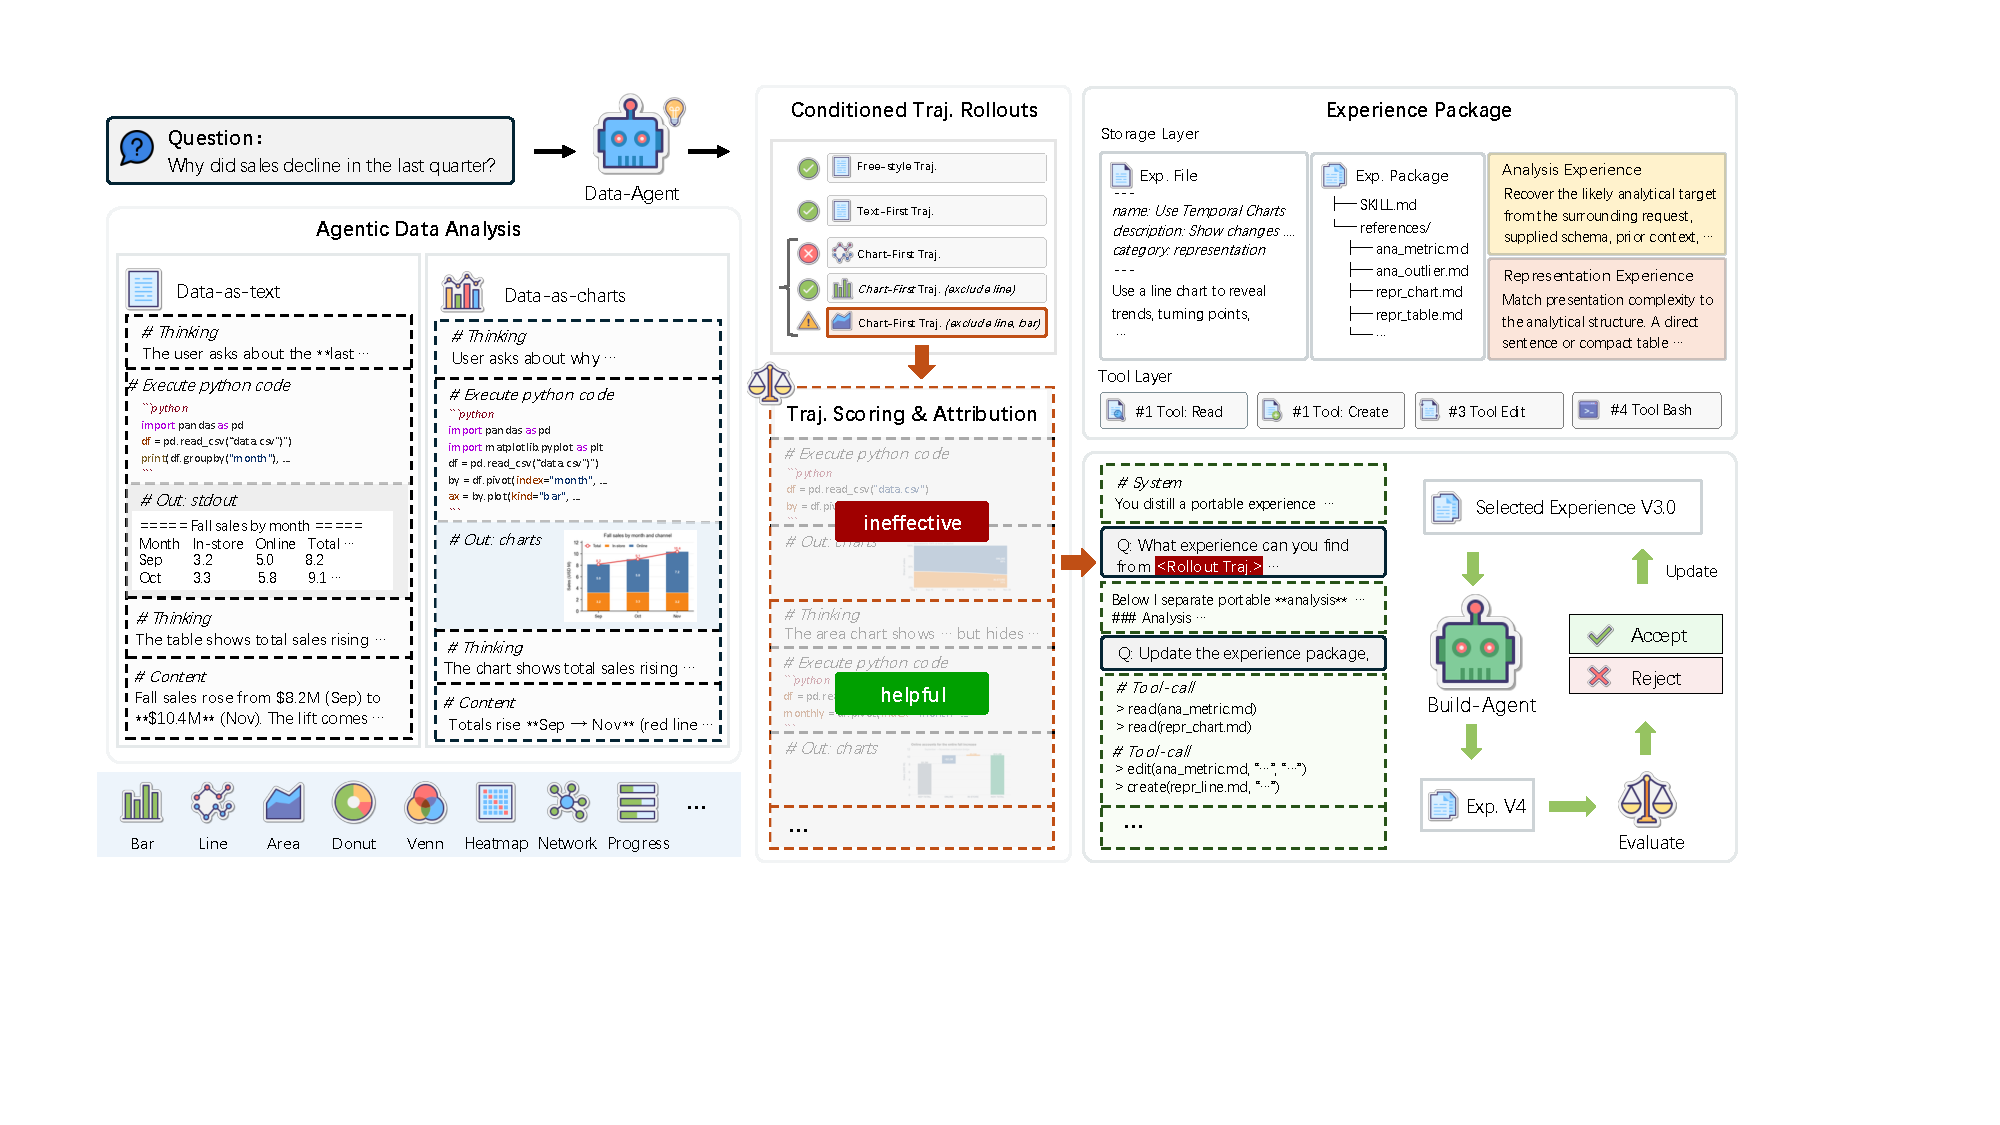
\includegraphics[width=0.92\linewidth]{figures/fig_main_v1.pdf}
  \caption{Overview of the experience-driven method for chart use in agentic data analysis.
    A data agent produces conditioned trajectories with different representation preferences, and a trajectory judge scores their outcomes and attributes intermediate decisions.
    A builder agent distills analysis and representation experiences into a validated experience package that guides downstream analysis.}
  \label{fig:method}
\end{figure}




\subsection{Experience Package}
\label{sec:experience-package}

\noindent\textbf{Storage and tool layers.}
The experience package consists of a storage layer and a tool layer.
The storage layer uses a file-system structure in which an entry document organizes independent experience documents.
Each document contains metadata fields such as \texttt{name}, \texttt{description}, and \texttt{category}, together with its experience content, which supports direct reading, editing, and versioning.

The tool layer provides \texttt{Read}, \texttt{Create}, \texttt{Edit}, and \texttt{Bash} for reading, creating, modifying, and managing experience documents.
The builder agent uses all four tools to maintain the package, whereas the data agent accesses experience only through \texttt{Read}.
Experience is loaded progressively.
The data agent first receives document metadata and then reads relevant content according to the current task and analysis state.

\noindent\textbf{Analysis and representation experiences.}
We extract two types of experience.
Analysis experience $\mathcal{E}_{\mathrm{ana}}$ summarizes how to select, organize, and verify analytical operations.
Representation experience $\mathcal{E}_{\mathrm{repr}}$ summarizes when to use text, charts, or hybrid representations and how to use them to advance subsequent analysis.
The two types are stored separately and updated and validated as one experience package.
We denote its $v$-th version by $\mathcal{E}^{(v)}=(\mathcal{E}_{\mathrm{ana}}^{(v)},\mathcal{E}_{\mathrm{repr}}^{(v)})$.

\subsection{Conditioned Trajectory Rollouts}
\label{sec:conditioned-rollouts}

We denote the $i$-th \probe{} by $p_i=(D_i,q_i,z_i,y_i^{\star})$, where the four elements represent the data, question, task context, and reference answer.
For each task, we generate multiple analysis trajectories under different representation conditions while holding the base agent, tools, and interaction budget fixed.
The trajectory generated under condition $\rho$ is denoted by $\tau_i^{\rho}$.
Each task yields a bundle of five trajectories,
\begin{equation}
\mathcal{B}_i=
\left\{
\tau_i^{\mathrm{U}},
\tau_i^{\mathrm{T}},
\tau_i^{\mathrm{C}_1},
\tau_i^{\mathrm{C}_2},
\tau_i^{\mathrm{C}_3}
\right\}.
\end{equation}
Here, $\tau_i^{\mathrm{U}}$ is an unconstrained rollout, $\tau_i^{\mathrm{T}}$ is a text-preferred rollout, and $\tau_i^{\mathrm{C}_k}$ for $k\in\{1,2,3\}$ are three chart-preferred rollouts.
These conditions change only the representation preference and do not restrict the analytical operations available to the agent.

To increase diversity among chart trajectories, we sequentially exclude chart types used by preceding chart-preferred rollouts.
The second rollout cannot reuse any chart type from the first, and the third cannot reuse types from either of the first two.
This constraint diversifies the visual analyses without assuming that charts outperform text or that any chart type is intrinsically superior.
The five trajectories from the same \probe{} form the basic unit for subsequent scoring and experience distillation.

\subsection{Trajectory Scoring and Attribution}
\label{sec:trajectory-attribution}

For each trajectory, a trajectory judge produces an outcome score and step-level attribution using the task question and reference answer $y_i^{\star}$.
The outcome score evaluates the final answer.
The attribution labels key steps as \texttt{Helpful}, \texttt{Ineffective}, or \texttt{Harmful}, and diagnoses the contributions of both analytical operations and representation choices.
Together, these signals indicate which behaviors the builder agent should retain or avoid.

\subsection{Experience Distillation and Validation}
\label{sec:experience-learning}

We split the experience-construction and validation sets by \probe{}, ensuring that all trajectories from the same task remain in the same split.
At each iteration, we sample $b$ tasks from the experience-construction set and provide their complete trajectory bundles, outcome scores, and step-level attributions to the builder agent.

Each update has two steps.
During insight induction, the builder agent compares trajectories and their attributions to identify transferable analysis and representation patterns.
During experience consolidation, it reads the current package and merges these patterns into existing documents or creates new analysis and representation experiences.

The builder agent edits the previously accepted package $\mathcal{E}^{(v-1)}$ and produces a candidate $\widetilde{\mathcal{E}}^{(v)}$.
Let $Q(\mathcal{E})$ denote validation performance with experience package $\mathcal{E}$.
The update rule is
\begin{equation}
\mathcal{E}^{(v)}=
\begin{cases}
\widetilde{\mathcal{E}}^{(v)},
& Q(\widetilde{\mathcal{E}}^{(v)})
>Q(\mathcal{E}^{(v-1)}),\\[4pt]
\mathcal{E}^{(v-1)},
& \text{otherwise}.
\end{cases}
\label{eq:experience-gate}
\end{equation}
The candidate is accepted only when validation performance strictly improves.
After multiple iterations, the final package $\mathcal{E}^{\star}$ is frozen for downstream tasks.

\subsection{Experience-Guided Analysis}
\label{sec:online}

For downstream tasks, the data agent uses the frozen package $\mathcal{E}^{\star}$.
The system first provides document metadata, after which the agent reads relevant experiences according to the question and current analysis state.
Analysis experience guides the selection and verification of analytical operations.
Representation experience guides whether intermediate results use text, charts, or both.
The base model parameters remain unchanged.
The external experience package guides chart use according to the task and analysis state, making charts part of the analytical process rather than a fixed preference or final presentation artifact.
Figure~\ref{fig:method} provides an overview of the full pipeline.

\section{Experiments}
\label{sec:experiments}

We evaluate our method on three benchmarks covering analytical report generation, long-horizon exploration, and exact-answer data analysis.
We first describe the benchmarks and evaluation protocol, then report the available results and retain incomplete runs as explicit \texttt{TBD} placeholders.

\subsection{Benchmarks}
\label{sec:benchmarks}

We use three benchmarks with complementary task forms and follow the evaluation protocol and metric computation defined by each benchmark.
\textbf{DAComp-DA} contains 100 open-ended tasks over potentially multi-table SQLite databases and requires reports with analysis, conclusions, and visualizations~\citep{lei2025dacomp}; we report Completeness, Accuracy, Insightfulness, Readability, Analytical Depth, Visualization, and Overall.
\textbf{DDR-Bench} evaluates long-horizon exploration without predefined queries~\citep{liu2026ddrbench}; we use its public 10-K setting over SEC disclosures from 100 companies and report Message-Wise accuracy, Trajectory-Wise accuracy, and Overall.
\textbf{DSBench} derives exact-answer tasks from ModelOff competitions with spreadsheet, text, and image inputs~\citep{jing2024dsbench}; its Data Analysis subset contains 40 challenges and approximately 466 questions, and we report Task-level Accuracy, Competition-level Accuracy, and Overall.

\subsection{Experimental Setup}
\label{sec:main-exp-setup}

We compare reported benchmark agents, a baseline agent reproduced in our common harness, and our method across Claude Opus 5, Claude Sonnet 5, GPT-5.6 Luna, GPT-5.6 Sol, DeepSeek V4.1 Flash, and HY4 Preview.
Within each backbone, the baseline and our method share the model version, decoding configuration, system instructions, data access, interaction budget, ReAct loop, Bash, Python, and SQL tools, stdout, stderr, and chart feedback; only our method reads the frozen experience package, so improvements cannot be attributed to plotting access alone.

All experience distillation uses only \probe{} and follows the conditioned trajectory rollout, trajectory scoring and attribution, and validation procedures in Section~\ref{sec:experience-learning}.
Source-data flags remain within a single \probe{} split, and all external benchmarks are held out from experience construction to prevent source leakage and assess transfer.
Each backbone constructs its experience package independently from the same initial structure, and the accepted version is frozen before external evaluation.

Each benchmark uses its official evaluator, namely DAComp-DA's official rubric and GSB suite, DDR-Bench's GPT-5-mini checker, and DSBench's answer-correctness procedure.
Methods share samples, judge prompts, and parameters within each benchmark, and reported prior results are compared only when splits and protocols match.
All core comparisons are paired, with clustered bootstrap confidence intervals at the task, company, and challenge levels, respectively.

\subsection{Main Results}
\label{sec:main-results}

We report each benchmark under its official metric and do not aggregate scores across incompatible scales.
Cells marked ``TBD'' are placeholders for incomplete runs or official evaluations, not estimates.

\noindent\textbf{DAComp-DA.}
Table~\ref{tab:dacomp-matrix} reports analytical report generation results.
We will report official Overall from \texttt{[A]} to \texttt{[B]}, together with changes in Completeness \texttt{[$\Delta$C]}, Accuracy \texttt{[$\Delta$A]}, and Visualization \texttt{[$\Delta$V]}.
Joint gains in content-correctness metrics and Visualization would indicate that visual representation supports analysis rather than surface presentation alone.

\noindent\textbf{DDR-Bench.}
Table~\ref{tab:ddr-matrix} reports long-horizon exploration results.
We will report Message-Wise accuracy \texttt{[X.X]} and Trajectory-Wise accuracy \texttt{[Y.Y]}, with Baseline-relative gains of \texttt{[$\Delta$X]} and \texttt{[$\Delta$Y]} points.
Larger Trajectory-Wise gains would indicate a stronger effect on long-horizon exploration and evidence synthesis, whereas gains in both metrics would indicate improvements in both local discovery and end-to-end coverage.

\noindent\textbf{DSBench.}
Table~\ref{tab:dsbench-matrix} reports exact-answer analysis results.
We will report Task-level Accuracy \texttt{[X.X]} and competition-macro Competition-level Accuracy \texttt{[Y.Y]}, with Baseline-relative gains of \texttt{[$\Delta$X]} and \texttt{[$\Delta$Y]} points.
Concurrent gains would indicate that improvements are not driven only by competitions containing more tasks.

\begin{table}[t]
  \caption{Results on \textit{DAComp-DA}.}
  \label{tab:dacomp-matrix}
  \centering
  \scriptsize
  \setlength{\tabcolsep}{2.5pt}
  \begin{tabular}{@{}>{\raggedright\arraybackslash}l>{\raggedright\arraybackslash}lccccccc@{}}
    \toprule
    Method & LLM Backbone & Completeness & Accuracy & Insightfulness & Readability & Analytical Depth & Visualization & Overall \\
    \midrule
    \multirow{2}{*}{\tabmethodreported{OpenHands}} & GPT-5 & 60.98 & 40.3 & 49.39 & 35.51 & 69.80 & 21.40 & 46.99 \\
      & DeepSeek-V3.1 & 49.88 & 33.25 & 41.66 & 36.00 & 33.20 & 11.00 & 33.87 \\
    % OpenHands & Qwen3-Coder & 33.42 & 21.21 & 25.06 & 20.00 & 13.73 & 4.80 & 24.28 \\
    \midrule
    \multirow{2}{*}{\tabmethodreported{DA-Agent}} & GPT-5 & 64.23 & 43.81 & 56.89 & 43.59 & 76.80 & 27.44 & 50.84 \\
      & DeepSeek-V3.1 & 48.74 & 32.97 & 42.43 & 37.25 & 35.00 & 11.45 & 34.33 \\
    % DA-Agent & Qwen3-Coder & 35.12 & 20.05 & 25.53 & 19.37 & 13.42 & 5.15 & 25.13 \\
    \midrule
    \multirow{4}{*}{\tabmethodbaseline}
      % & Claude Opus 5 & TBD & TBD & TBD & TBD & TBD & TBD & TBD \\
      & Claude Sonnet 5 & 70.27 & 52.55 & 68.85 & 90.80 & 89.00 & 62.80 & 69.84 \\
      & GPT-5.6 Luna & 66.21 & 46.61 & 65.45 & 83.83 & 80.74 & 7.66 & 54.32 \\
      & GPT-5.6 Sol & 71.74 & 58.04 & 72.42 & 94.60 & 93.00 & 61.80 & 73.24 \\
      & DeepSeek V4.1 Flash & 83.91 & 67.80 & 81.77 & 98.0 & 94.44 & 75.72 & 82.23 \\
      % & HY4 Preview & 78.55 & 60.38 & 74.39 & 96.74 & 94.78 & 66.52 & 79.40 \\
    \midrule
    \multirow{4}{*}{\method{}}
      % & Claude Opus 5 & TBD & TBD & TBD & TBD & TBD & TBD & TBD \\
      & Claude Sonnet 5 & TBD & TBD & TBD & TBD & TBD & TBD & TBD \\
      & GPT-5.6 Luna & 68.10 & 51.18 & 65.24 & 82.83 & 85.00 & 27.61 & 59.78 \\
      & GPT-5.6 Sol & TBD & TBD & TBD & TBD & TBD & TBD & TBD \\
      & DeepSeek V4.1 Flash & TBD & TBD & TBD & TBD & TBD & TBD & TBD \\
      % & HY3 & TBD & TBD & TBD & TBD & TBD & TBD & TBD \\
    \bottomrule
  \end{tabular}

  \benchmarkstacksep

  \begin{minipage}[t]{0.48\textwidth}
    \centering
    \captionof{table}{Results on \textit{DDR-Bench}.}
    \label{tab:ddr-matrix}
    \scriptsize
    \setlength{\tabcolsep}{2.5pt}
    \begin{tabular}{@{}>{\raggedright\arraybackslash}l>{\raggedright\arraybackslash}lccc@{}}
      \toprule
      Method & LLM & \makecell{Msg.\\\headpct} & \makecell{Traj.\\\headpct} & \makecell{Overall\\\headpct} \\
      \midrule
      \multirow{4}{*}{\tabmethodreported{ReAct}} & Claude Sonnet 4.5 & 77.61 & 60.58 & 69.10 \\
        & GPT-5.1 & 37.12 & 44.25 & 40.69 \\
        & GPT-5.2 & 44.89 & 41.09 & 42.99 \\
        & DeepSeek V3.2 & 60.08 & 38.15 & 49.12 \\
      % ReAct & GLM-4.6 & 60.31 & 36.02 & 48.17 \\
      % ReAct & Kimi K2 & 51.06 & 30.84 & 40.95 \\
      % ReAct & MiniMax M2 & 44.17 & 26.88 & 35.53 \\
      \midrule
      \multirow{4}{*}{\tabmethodbaseline}
        % & Claude Opus 5 & TBD & TBD & TBD \\
        & Claude Sonnet 5 & 61.2 & 52.2 & 56.7 \\
        & GPT-5.6 Luna & 44.5 & 45.1 & 44.8 \\
        & GPT-5.6 Sol & 60.2 & 58.5 & 59.4 \\
        & DeepSeek V4.1 Flash & 64.2 & 59.0 & 61.6 \\
        % & HY4 Preview & TBD & TBD & TBD \\
      \midrule
      \multirow{4}{*}{\method{}}
        % & Claude Opus 5 & TBD & TBD & TBD \\
        & Claude Sonnet 5 & TBD & TBD & TBD \\
        & GPT-5.6 Luna & TBD & TBD & TBD \\
        & GPT-5.6 Sol & TBD & TBD & TBD \\
        & DeepSeek V4.1 Flash & TBD & TBD & TBD \\
        % & HY4 Preview & TBD & TBD & TBD \\
      \bottomrule
    \end{tabular}
  \end{minipage}\hfill
  \begin{minipage}[t]{0.48\textwidth}
    \centering
    \captionof{table}{Results on \textit{DSBench}.}
    \label{tab:dsbench-matrix}
    \scriptsize
    \setlength{\tabcolsep}{2.5pt}
    \begin{tabular}{@{}>{\raggedright\arraybackslash}l>{\raggedright\arraybackslash}lccc@{}}
      \toprule
      Method & LLM & \makecell{Task\\\headpct} & \makecell{Comp.\\\headpct} & \makecell{Overall\\\headpct} \\
      \midrule
      % \textit{Human} & \na & 64.06 & 67.33 & 65.70 \\
      % Model-only & GPT-3.5 & 20.39 & 11.85 & 16.12 \\
      % Model-only & GPT-4o & 28.11 & 19.26 & 23.69 \\
      \multirow{2}{*}{\tabmethodreported{Code Inter.}} & GPT-3.5 & 11.16 & 8.23 & 9.70 \\
        & GPT-4o & 23.82 & 22.65 & 23.24 \\
      \midrule
      \multirow{2}{*}{\tabmethodreported{AutoGen}} & GPT-3.5 & 20.82 & 13.80 & 17.31 \\
        & GPT-4o & 34.12 & 26.72 & 30.42 \\
      \midrule
      \multirow{4}{*}{\tabmethodbaseline}
        % & Claude Opus 5 & TBD & TBD & TBD \\
        & Claude Sonnet 5 & 88.47 & 88.42 & 88.45 \\
        & GPT-5.6 Luna & 75.11 & 73.84 & 74.47 \\
        & GPT-5.6 Sol & 89.9 & 89.4 & 89.7 \\
        & DeepSeek V4.1 Flash & TBD & TBD & TBD \\
        % & HY4 Preview & 92.70 & 91.19 & 91.95 \\
      \midrule
      \multirow{4}{*}{\method{}}
        % & Claude Opus 5 & TBD & TBD & TBD \\
        & Claude Sonnet 5 & TBD & TBD & TBD \\
        & GPT-5.6 Luna & 76.72 & 76.25 & 76.49 \\
        & GPT-5.6 Sol & TBD & TBD & TBD \\
        & DeepSeek V4.1 Flash & TBD & TBD & TBD \\
        % & HY4 Preview & TBD & TBD & TBD \\
      \bottomrule
    \end{tabular}
  \end{minipage}
  \vspace{-4pt}
\end{table}


\subsection{Ablation Studies and Mechanism Analysis}
\label{sec:ablations}

We conduct all ablation studies on DAComp-DA using the same backbone, ReAct loop, tool interface, interaction budget, and official evaluator.
We report Acc., Vis., and Overall, which respectively measure analytical correctness, visual presentation quality, and aggregate performance.
Unless otherwise stated, the ablations change only the component under study.
Tables~\ref{tab:ablation-construction}--\ref{tab:ablation-experience-types} report the currently available results.

\begin{wraptable}{r}{0.50\textwidth}
  \vspace{-8pt}
  \centering
  \scriptsize
  \setlength{\tabcolsep}{5pt}
  \begin{minipage}{\linewidth}
    \centering
    \captionof{table}{Ablation to experience construction, comparing baseline and one-step distillation (OSD).}
    \label{tab:ablation-construction}
    \begin{tabular}{@{}lccc@{}}
      \toprule
      Variant & Acc.~\headpct & Vis.~\headpct & Overall~\headpct \\
      \midrule
      Baseline & 46.61 & 7.66 & 54.32 \\
      OSD & 51.26 & 26.35 & 61.10 \\
      \method{} & 51.18 & 27.61 & 59.78 \\
      \bottomrule
    \end{tabular}
  \end{minipage}

  \floatstacksep

  \begin{minipage}{\linewidth}
    \centering
    \captionof{table}{Ablation to conditioned rollouts (CR) and validation gating (VG) in iterative distillation.}
    \label{tab:ablation-iterative}
    \begin{tabular}{@{}lccc@{}}
      \toprule
      Variant & Acc.~\headpct & Vis.~\headpct & Overall~\headpct \\
      \midrule
      w/o CR & TBD & TBD & TBD \\
      w/o VG & TBD & TBD & TBD \\
      \method{} & TBD & TBD & TBD \\
      \bottomrule
    \end{tabular}
  \end{minipage}

  \floatstacksep

  \begin{minipage}{\linewidth}
    \centering
    \captionof{table}{Ablation to experience categories, retaining analysis experience only (Ana.) or representation experience only (Rep.).}
    \label{tab:ablation-experience-types}
    \begin{tabular}{@{}lccc@{}}
      \toprule
      Variant & Acc.~\headpct & Vis.~\headpct & Overall~\headpct \\
      \midrule
      Ana. & TBD & TBD & TBD \\
      Rep. & TBD & TBD & TBD \\
      \method{} & TBD & TBD & TBD \\
      \bottomrule
    \end{tabular}
  \end{minipage}
\end{wraptable}

\noindent\textbf{Experience construction strategies.}
Table~\ref{tab:ablation-construction} compares the baseline, one-step distillation, and our method. One-step distillation constructs a frozen package from the complete trajectory corpus in one builder call, whereas our method updates the package over successive batches with validation. The current runs cover 100 tasks for one-step distillation and 92 for our method; their similar Acc., higher Overall for one-step distillation, and higher Vis. for our method remain preliminary until evaluation on a matched task set.

\noindent\textbf{Mechanisms of iterative distillation.}
Table~\ref{tab:ablation-iterative} isolates conditioned trajectory evidence and validation-based package selection. The rollout-free variant receives the same questions, data descriptions, and reference insights without trajectories, outcome scores, or step-level attributions, while the ungated variant retains every update; results remain \texttt{TBD}.

\noindent\textbf{Analysis and representation experiences.}
Table~\ref{tab:ablation-experience-types} compares the complete package with analysis-only and representation-only variants obtained by retaining documents from only the corresponding category. Acc. measures effects on analytical correctness, while Vis. measures effects on visual evidence and presentation; results remain \texttt{TBD}.

\noindent\textbf{Tool use and optimization dynamics.}
Figure~\ref{fig:tool-use-ablation} will compare ReAct rounds, Bash calls, and experience-read calls for the baseline, one-step distillation, and our method, with results currently \texttt{TBD}. Figure~\ref{fig:experience-convergence} reports the available optimization trajectory, where validation filters lower-scoring candidates and maintains a non-decreasing trajectory for the retained experience package.

\pairedfigrow{%
  \pairedfigplaceholder{Tool-use analysis pending}%
  \pairedfigcaption[fig:tool-use-ablation]{Tool-use on DAComp-DA (TBD). ReAct, Bash, and experience reads.}%
}{%
  \pairedfiginclude{figures/experience_distillation_convergence_v2.pdf}%
  \pairedfigcaption[fig:experience-convergence]{Validation scores during experience-package distillation.}%
}

\WFclear

\section{Related Work}
\label{sec:related}

\subsection{Data agents.}
LLM-driven data agents increasingly follow a plan--execute--observe--revise paradigm.
DS-Agent couples language-model reasoning with an executable analysis environment and retrieves historical cases to support data-science problem solving; Data Interpreter organizes complex tasks as dynamic directed acyclic graphs, advancing analysis through hierarchical decomposition and code execution; AIDE models machine-learning solution development as tree search in code space; DS-STAR handles heterogeneous data-analysis tasks via iterative planning and plan-sufficiency verification; and AutoKaggle and related systems adopt multi-agent division of labor for data understanding, solution planning, program development, and result review~\citep{guo2024dsagent,hong2025datainterpreter,jiang2025aide,nam2025dsstar,li2025autokaggle}.
Meanwhile, DeepAnalyze targets end-to-end coverage of data preparation, analysis, modeling, visualization, and report generation through specialized training, and InsightBench extends evaluation to open-ended, multi-step business insight generation~\citep{zhang2025deepanalyze,sahu2025insightbench}.
Although these lines of work continue to advance planning, search, collaboration, and training mechanisms, their analysis loops still rely predominantly on textual representations of structured data and on code-execution outputs as intermediate feedback.
Some systems can generate charts, but few isolate whether agents inspect self-generated charts and leverage the visual patterns they reveal to form hypotheses and steer subsequent analysis.
We focus on how visual evidence enters the intermediate reasoning loop of data agents.

\subsection{Charts in data analysis.}
In parallel with data agents, research on charts has made substantial progress in chart generation, understanding, and representation choice.
For chart generation, LIDA established a pipeline from data summaries and visualization goals to plotting code; MatPlotAgent uses rendered visual feedback to iteratively repair visualization programs; ChartMimic, AMACE, and MultiVis-Agent further improve reliability through cross-modal reconstruction, multi-agent collaboration, and iterative optimization; and ChartOptimiser shows that chart design should adapt to the analytical task at hand~\citep{dibia2023lida,yang2024matplotagent,yang2025chartmimic,namgoong2025amace,lu2026multivisagent,wang2025chartoptimiser}.
For chart understanding, UniChart, ChartLlama, and ChartBench advance chart reading and reasoning via specialized training and large-scale evaluation; DePlot, MatCha, and TinyChart improve numerical analysis through derendering, structural recovery, and programmatic reasoning; and ChartAgent and Charts-of-Thought demonstrate that visual tools combined with structured reasoning can strengthen complex chart analysis~\citep{masry2023unichart,han2023chartllama,xu2023chartbench,liu2023deplot,liu2023matcha,zhang2024tinychart,kaur2026chartagent,das2025chartsofthought}.
Building on this foundation, FRES, Format Matters, and TableDART study effectiveness differences and dynamic selection among textual, image, and chart representations, while systems such as EvidFuse construct visual evidence on demand during analysis or reporting~\citep{zhou2025fres,ho2026formatmatters,xing2026tabledart,lin2026evidfuse}.
However, existing work typically generates user-specified charts, interprets externally provided charts, or selects among pre-existing representations; it has not systematically studied how data agents jointly choose analytical operations and text or chart representations, and use self-generated charts as intermediate evidence for discovering patterns and advancing subsequent analysis.

\section{Conclusion}
\label{sec:conclusion}

We study how charts can serve as internal epistemic actions rather than end-of-analysis illustrations.
\probe{} shows that current data agents can complete end-to-end analysis through self-generated charts, yet often fail to turn plotting-tool access into consistent gains, and exhibit strong model-specific representation preferences when text and charts are both available.
Task slices indicate complementary roles: charts support trends and pattern discovery, whereas text better preserves precise, verifiable evidence.
Our method distills analysis and representation experiences from conditioned trajectory rollouts with outcome scores and step-level attributions, learning both what evidence to construct and how to represent and use it without fixed representation-selection rules.
Experiments on held-out benchmarks indicate that this experience-driven chart use improves over matched baselines, supporting the view that representation choice is part of the analytical policy rather than a cosmetic output.


\bibliography{iclr2027_conference}
\bibliographystyle{iclr2027_conference}

\appendix

\section{Complete \probe{} Slice Results}
\label{app:slices}

Tasks may have multiple analytical-operation labels, while each task has one primary cognitive-operation label.
Low-$n$ rows are included for completeness and should not be interpreted as stable representation effects.

\begin{table}[h]
  \caption{Scores by analytical operation.}
  \label{tab:operation-slices}
  \centering
  \scriptsize
  \setlength{\tabcolsep}{3.5pt}
  \begin{tabular}{lrrrrr}
    \toprule
    Slice & $n$ & No-tool & Text & Chart & Free-style \\
    \midrule
    Filtering             & 109 & 0.257 & 0.752 & 0.752 & 0.755 \\
    Feature derivation    & 116 & 0.257 & 0.739 & 0.752 & 0.744 \\
    Aggregation           & 163 & 0.305 & 0.773 & 0.791 & 0.781 \\
    Normalization         &  21 & 0.143 & 0.571 & 0.512 & 0.583 \\
    Sorting               &  22 & 0.284 & 0.818 & 0.830 & 0.784 \\
    Alignment/joining     &   8 & 0.188 & 0.719 & 0.563 & 0.719 \\
    Temporal change       &  37 & 0.237 & 0.757 & 0.838 & 0.757 \\
    Distributional stats. &   1 & 1.000 & 1.000 & 1.000 & 1.000 \\
    Statistical inference &  10 & 0.200 & 0.925 & 0.900 & 0.900 \\
    Forecasting           &   3 & 0.000 & 1.000 & 1.000 & 1.000 \\
    \bottomrule
  \end{tabular}
\end{table}

\begin{table}[h]
  \caption{Scores by primary cognitive operation.}
  \label{tab:cognitive-slices}
  \centering
  \scriptsize
  \setlength{\tabcolsep}{3.5pt}
  \begin{tabular}{lrrrrr}
    \toprule
    Slice & $n$ & No-tool & Text & Chart & Free-style \\
    \midrule
    Lookup                    & 12 & 0.146 & 0.604 & 0.521 & 0.521 \\
    Scan and selection        & 24 & 0.219 & 0.958 & 0.958 & 0.958 \\
    Comparative judgment      & 69 & 0.366 & 0.801 & 0.783 & 0.808 \\
    Pattern recognition       & 54 & 0.306 & 0.769 & 0.833 & 0.764 \\
    Relational explanation    & 17 & 0.221 & 0.706 & 0.735 & 0.765 \\
    Multidimensional integration & 20 & 0.150 & 0.575 & 0.650 & 0.600 \\
    Conditional reasoning     &  4 & 0.813 & 1.000 & 0.750 & 1.000 \\
    \bottomrule
  \end{tabular}
\end{table}

\section{Items Required Before Submission}
\label{app:pending}

The final manuscript still requires: confirmation that the method terminology and \probe{} do not conflict with prior names; final probe and framework artwork; a qualitative trajectory figure; pseudocode for experience distillation and experience-guided analysis; completed external-benchmark and ablation results with statistical tests; judge robustness and human-agreement checks; representative experience entries and full prompts; and compute, cost, and implementation details.

\end{document}
